% Compile with: lualatex double_chaotic_validation.tex (twice)
\documentclass[a4paper,11pt]{ltjsarticle}

\usepackage{luatexja-fontspec}
\usepackage{amsmath,amssymb}
\usepackage{booktabs}
\usepackage{graphicx}
\usepackage{geometry}
\usepackage{siunitx}
\usepackage{xcolor}
\usepackage{hyperref}
\usepackage{enumitem}
\usepackage{float}
\usepackage{caption}
\usepackage{longtable}

\geometry{left=23mm,right=23mm,top=23mm,bottom=25mm}
\graphicspath{{../figures/}{../ode_validation/}}
% Auto-generated by compare_double_chaotic.py. Do not edit by hand.
\newcommand{\RunEfolds}{86.091795}
\newcommand{\SlowRollEfolds}{84}
\newcommand{\EfoldRelativeDifference}{0.024902318}
\newcommand{\EfoldRelativePercent}{2.4902318}
\newcommand{\InitialHLattice}{4.8085037e-05}
\newcommand{\InitialHAnalytic}{4.8058992e-05}
\newcommand{\InitialHRelativeDifference}{0.00054195074}
\newcommand{\InitialHRelativePercent}{0.054195074}
\newcommand{\InitialW}{-0.99855592}
\newcommand{\FinalW}{-0.33300953}
\newcommand{\FinalEpsilonH}{1.0004855}
\newcommand{\TransitionNLattice}{44.860808}
\newcommand{\TransitionNAnalytic}{44.014511}
\newcommand{\TransitionRelativePercent}{1.9227685}
\newcommand{\FriedmannMaximum}{0.00019854103}
\newcommand{\HSRRms}{0.017958422}
\newcommand{\HSRRmsPercent}{1.7958422}
\newcommand{\PhiSRRms}{0.014097206}
\newcommand{\PhiSRRmsPercent}{1.4097206}
\newcommand{\PsiSRRms}{0.020186943}
\newcommand{\PsiSRRmsPercent}{2.0186943}
\newcommand{\ComparisonNMin}{1.0002492}
\newcommand{\ComparisonNMax}{81.270037}
\newcommand{\GradientFractionMaximum}{1.0059084e-05}
\newcommand{\InitialPotentialFraction}{0.99891698}
\newcommand{\InitialKineticFraction}{0.00054155235}
\newcommand{\InitialGradientFraction}{0.00054146626}
\newcommand{\InhomogeneousFractionMaximum}{2.0100236e-05}
\newcommand{\BDPhiWeightedRatio}{0.99692652}
\newcommand{\BDPsiWeightedRatio}{1.0078206}
\newcommand{\HorizonPsiMeanRatio}{1.0041073}
\newcommand{\HorizonPsiMedianRatio}{0.99467499}
\newcommand{\HorizonCrossingNMin}{1.9533102}
\newcommand{\HorizonCrossingNMax}{4.6139843}
\newcommand{\ParsevalPhi}{1.5881417e-05}
\newcommand{\ParsevalPsi}{1.5549136e-05}
\newcommand{\ODEFieldRms}{2.3858652e-07}
\newcommand{\ODEVelocityRms}{3.2391071e-05}
\newcommand{\ODEHomogeneousHRms}{6.5902934e-05}


\hypersetup{
  colorlinks=true,
  linkcolor=blue!55!black,
  citecolor=blue!55!black,
  urlcolor=blue!55!black,
  pdftitle={MultifieldInflationLattice 2026-08-18 run validation},
  pdfauthor={Validation report generated from the recorded run}
}
\sisetup{scientific-notation=true,round-mode=figures,round-precision=4}
\setlist[itemize]{leftmargin=2em,itemsep=0.2em,topsep=0.3em}
\captionsetup{font=small,labelfont=bf}

\newcommand{\code}[1]{\texttt{#1}}
\newcommand{\pass}{\textcolor{green!45!black}{PASS}}
\newcommand{\cF}{\mathcal{C}_{\mathrm F}}

\title{二場二次ポテンシャル格子シミュレーションの\\
解析的 slow-roll 近似および独立 ODE との比較}
\author{対象: \code{MultifieldInflationLattice} 2026年8月18日実行結果}
\date{2026年8月24日}

\begin{document}
\maketitle

\begin{abstract}
本稿は、2026年8月18日に開始され正常終了した二場二次ポテンシャルの格子計算
\code{two\_field\_quadratic\_20260818T205254Z\_6c5330a9ab54}
について、背景発展とゆらぎ初期化が理論的期待に整合するかを検証する。
比較対象は、(i) 解析的 slow-roll 近似、(ii) Friedmann 方程式と
stress-energy の厳密恒等式、(iii) 実装から独立した adaptive
Dormand--Prince 5(4) ODE、(iv) Bunch--Davies 初期スペクトル、
(v) Parseval 恒等式である。選定した全検査は \pass となった。
初期 Hubble 率の差は \SI{\InitialHRelativePercent}{\percent}、
総 e-fold 数の差は \SI{\EfoldRelativePercent}{\percent}、
最大 Friedmann 残差は \num{\FriedmannMaximum} であり、設定許容値
$10^{-3}$ を下回った。したがって本実装は、少なくとも単一の
$32^3$ 格子・単一 seed における背景部門、真空ゆらぎ初期化および
FFT 規格化について、double-chaotic inflation の理論的挙動を再現する。
ただし本結果は連続極限、有限体積独立性、seed ensemble、および曲率摂動の
完全な精度保証ではない。
\end{abstract}

\section{目的と検証範囲}

自己重力を含む非一様二場系には、全発展を覆う有用な初等関数の閉形式解はない。
したがって本稿でいう「解析比較」は厳密解との一点比較ではなく、
解析的 slow-roll 予測、厳密な連続方程式の恒等式、独立な高精度 ODE 数値解を
組み合わせた検証である。目的はコード全体の数学的証明ではなく、8月18日の
出力が次の主張を支持するかを判定することである。

\begin{itemize}
  \item 重い場から軽い場へ支配成分が交代する二段階背景発展を再現する。
  \item 格子平均場が連続 Klein--Gordon 方程式と一致する。
  \item Friedmann 拘束、エネルギーおよび圧力の関係が設定精度内で成立する。
  \item 初期真空ゆらぎと場スペクトルの規格化が解析的期待に一致する。
\end{itemize}

\subsection{「複素場」という表現について}

メタデータの action は
\code{canonical\_real\_scalar\_fields\_flat\_FLRW\_v1} であり、実装上は
二つの正準実スカラー場である。形式的に
$\Phi=(\phi+i\psi)/\sqrt{2}$ とまとめることはできるが、
$m_\phi\ne m_\psi$ のため
\begin{equation}
 V=\frac{m_\phi^2+m_\psi^2}{2}|\Phi|^2
  +\frac{m_\phi^2-m_\psi^2}{4}\left(\Phi^2+\Phi^{*2}\right)
\end{equation}
となり、$U(1)$ 回転対称性はない。本稿では「質量の異なる二実成分」、
または同値に「異方的で $U(1)$ が明示的に破れた複素スカラー場」と解釈する。

\section{モデル、連続方程式および計算条件}

換算 Planck 単位 $M_{\mathrm{Pl}}=1$ を用い、ポテンシャルを
\begin{equation}
 V(\phi,\psi)=\frac12m_\phi^2\phi^2+\frac12m_\psi^2\psi^2
\end{equation}
とする。平坦 FLRW 背景上の連続方程式は
\begin{align}
 \ddot\phi_I+3H\dot\phi_I-\frac{1}{a^2}\nabla^2\phi_I+m_I^2\phi_I&=0,\\
 H^2&=\frac{\rho}{3},\\
 \dot H&=-\frac12(\rho+p),
\end{align}
である。格子平均量に対して
\begin{align}
 \rho &= K+G+V,\\
 p &= K-\frac13G-V,\\
 K&=\frac12\sum_I\langle\dot\phi_I^2\rangle,\qquad
 G=\frac{1}{2a^2}\sum_I\langle|\nabla\phi_I|^2\rangle
\end{align}
が成立する。コードでは周期境界の7点2次差分 Laplacian と2次精度
leapfrog を使用する。場方程式とスケール因子方程式は
\code{src/Dynamics.jl}、エネルギー定義は
\code{src/observables/Energy.jl}、物理単位への変換は
\code{src/observables/Background.jl} に実装されている。

\begin{table}[H]
\centering
\caption{解析対象runの主要設定。}
\begin{tabular}{ll}
\toprule
項目 & 設定値 \\
\midrule
場と質量 & $\phi,\psi$; $m_\phi=9\times10^{-6}$, $m_\psi=10^{-6}$ \\
初期平均場 & $(\phi_0,\psi_0)=(13,13)$ \\
初期平均速度 & $(10^{-10},0)$ \\
格子 & $32^3$, $L=2$, 周期境界 \\
空間差分 & second-order 7-point Laplacian \\
時間積分 & leapfrog, timestep factor $0.01$ \\
ゆらぎ & Bunch--Davies, seed $8$, effective mass 無効 \\
終了条件 & $\epsilon_H\geq1$ \\
Friedmann warning / error & $10^{-6}$ / $10^{-3}$ \\
run status & completed; end reason: \code{epsilon\_H\_reached} \\
\bottomrule
\end{tabular}
\end{table}

\section{解析的比較と判定方法}

\subsection{二場 slow-roll 解}

slow-roll 近似では
\begin{equation}
 3H\dot\phi_I\simeq-m_I^2\phi_I,qquad
 H^2\simeq\frac{V}{3}.
\end{equation}
$u=\psi/\psi_0$ および
$r=m_\phi^2/m_\psi^2=81$ を導入すると、背景軌道は
\begin{align}
 \psi_{\mathrm{SR}}(u)&=\psi_0u,\\
 \phi_{\mathrm{SR}}(u)&=\phi_0u^r,\\
 N_{\mathrm{SR}}(u)&=
 \frac{\phi_0^2(1-u^{2r})+\psi_0^2(1-u^2)}{4},\\
 H_{\mathrm{SR}}(u)&=
 \sqrt{\frac{m_\phi^2\phi_{\mathrm{SR}}^2+m_\psi^2\psi_{\mathrm{SR}}^2}{6}}.
\end{align}
さらに
\begin{equation}
 \epsilon_V=2\frac{m_\phi^4\phi^2+m_\psi^4\psi^2}
 {(m_\phi^2\phi^2+m_\psi^2\psi^2)^2}
\end{equation}
を用い、$\epsilon_V=1$ の根を解析曲線の終了点とした。数値runは
$\epsilon_H=1$ で終了するため、終了近傍の差はslow-roll近似の破れを含む。

点ごとの相対誤差は場がゼロに近づくと不安定になる。このため
$N\geq1$, $\epsilon_H<0.1$, $\Omega_G<10^{-3}$ の比較区間で
\begin{equation}
 E_X=\left[
 \frac{\langle(X_{\mathrm{lat}}-X_{\mathrm{ref}})^2\rangle}
 {\langle X_{\mathrm{ref}}^2\rangle}
 \right]^{1/2}
\end{equation}
を使用した。初期の静止条件からslow-roll attractorへ入る過渡期、
場空間の曲がり、および終了近傍は近似誤差が増える領域として扱う。

\subsection{内部拘束と独立 ODE}

Friedmann 残差は
\begin{equation}
 \cF=\frac{|H^2-\rho/3|}
 {\max(H^2,\rho/3,\rho_{\mathrm{floor}})}
\end{equation}
とした。$\rho=K+G+V$ などの代数恒等式は出力整合性検査であり、
単独では独立な物理検証ではない。一方、$H$ は時間発展したスケール因子から
得られるため、$H^2$ と $\rho/3$ の比較は有用な拘束検査である。

平均 Laplacian は周期境界で消え、二次ポテンシャルの勾配は線形なので、
格子平均場は厳密に
\begin{equation}
 \ddot{\bar\phi}_I+3H_{\mathrm{lat}}(t)\dot{\bar\phi}_I
 +m_I^2\bar\phi_I=0
\end{equation}
を満たす。これを Julia 実装をimportしない Python の adaptive
Dormand--Prince 5(4) で積分した。また、平均場エネルギーから $H$ を再計算する
自己無撞着な一様場 ODE も併記した。前者は平均場運動方程式、後者は
ゆらぎエネルギーが小さい範囲の背景膨張を検査する。

\subsection{ゆらぎスペクトル}

初期化でeffective massを無効にしているため、Bunch--Davies期待値は
\begin{equation}
 \Delta_{\delta\phi_I}^2(k)=\frac{k^2}{4\pi^2a_0^2}
\end{equation}
である。単一乱数実現のshell powerには有限モード散乱があるため、
mode-weighted平均と概算 $\sqrt{2/n_{\mathrm{modes}}}$ の散乱幅を用いた。
また、全モードがHubble crossingした後の軽い場について
\begin{equation}
 \mathcal P_{\delta\psi}(k)\simeq
 \left(\frac{H_*}{2\pi}\right)^2,\qquad k=a_*H_*
\end{equation}
と比較した。最後に、スペクトル和から再構成した分散と実空間分散を比較し、
FFT規格化を検査した。多場の曲率・等曲率摂動の一般論については
Ref.~\cite{Gordon2001}を参照されたい。

\section{結果}

\subsection{背景発展と二段階inflation}

初期平均場ポテンシャルから
$H_{\mathrm{SR}}(0)=\num{\InitialHAnalytic}$、格子出力は
$H(0)=\num{\InitialHLattice}$ であり、差は
\SI{\InitialHRelativePercent}{\percent} である。初期エネルギー比は
$\Omega_V=\num{\InitialPotentialFraction}$,
$\Omega_K=\num{\InitialKineticFraction}$,
$\Omega_G=\num{\InitialGradientFraction}$ であり、初期の小差は
真空ゆらぎの運動・勾配エネルギーで説明できる。

図\ref{fig:background}に示すように、$m_\phi/m_\psi=9$ の重い
$\phi$ が先に減少し、軽い $\psi$ が後半を支配する。平均場ポテンシャルが
等しくなる時刻は、slow-roll予測 $N=\TransitionNAnalytic$ に対して
格子では $N=\TransitionNLattice$ であり、差は
\SI{\TransitionRelativePercent}{\percent} である。
総e-fold数は解析近似 $N=\SlowRollEfolds$、格子
$N=\RunEfolds$ で、差は \SI{\EfoldRelativePercent}{\percent} となった。
比較区間における規格化RMS差は
$E_H=\SI{\HSRRmsPercent}{\percent}$,
$E_\phi=\SI{\PhiSRRmsPercent}{\percent}$,
$E_\psi=\SI{\PsiSRRmsPercent}{\percent}$ である。

終了点では $\epsilon_H=\FinalEpsilonH$、$w=\FinalW$ であり、
$\epsilon_H=1$ と $w=-1/3$ の関係を再現した。解析的slow-roll曲線は
終了近傍で破れるため、この領域の偏差を格子誤差とは判定しない。

\begin{figure}[p]
\centering
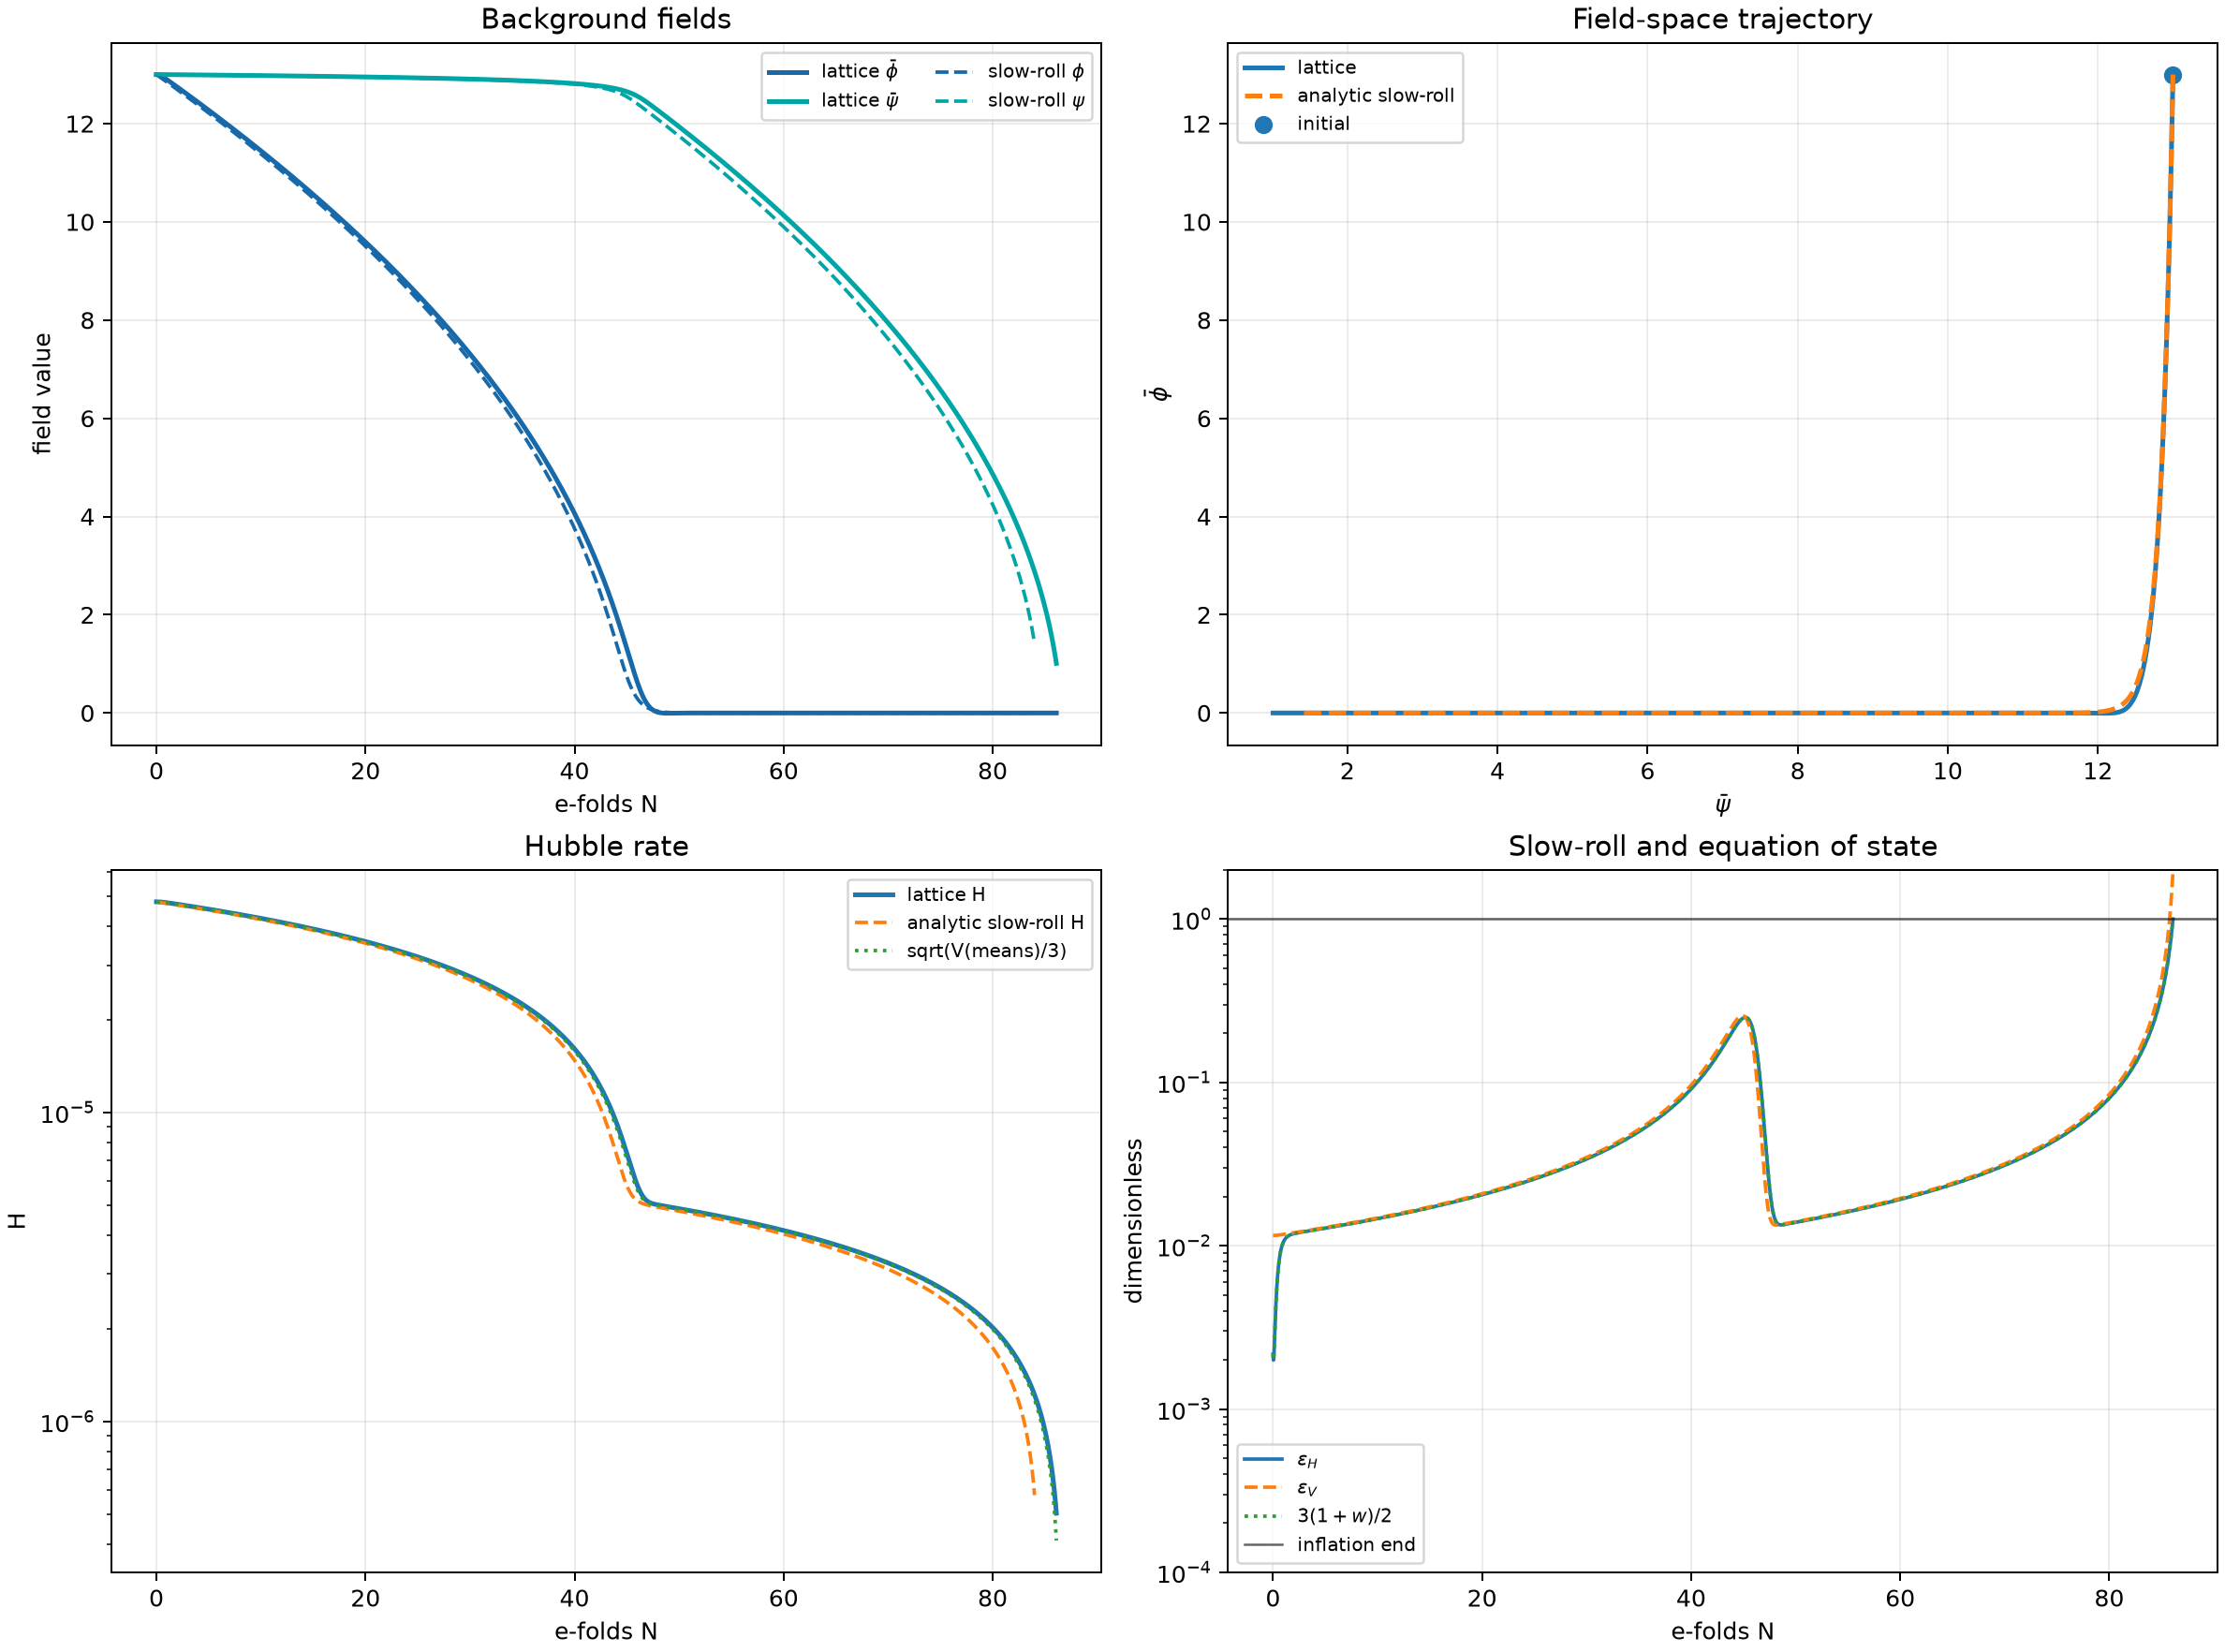
\includegraphics[width=0.98\textwidth]{background_vs_analytic.png}
\caption{格子平均背景と解析的slow-roll近似。左上は二場の時間発展、右上は場空間軌道、左下はHubble率、右下はslow-roll量と状態方程式の関係を示す。}
\label{fig:background}
\end{figure}

\subsection{エネルギー、拘束条件、独立ODE}

slow-roll比較区間の最大勾配比は
$\Omega_G^{\max}=\num{\GradientFractionMaximum}$ であり、背景比較が
非一様勾配に支配されていない。最大 Friedmann 残差
$\cF^{\max}=\num{\FriedmannMaximum}$ は error tolerance $10^{-3}$ 以下である。
一方、warning tolerance $10^{-6}$ は超えており、残差が機械精度であると
主張するものではない。エネルギー和と圧力分解の最大相対差はそれぞれ
$6.2\times10^{-16}$ と $6.6\times10^{-16}$ であった。

独立ODEの平均場規格化RMS差は \num{\ODEFieldRms}、平均速度は
\num{\ODEVelocityRms} である。自己無撞着な一様場ODEと格子Hubble率の
診断差は \num{\ODEHomogeneousHRms} であり、ゆらぎ・勾配エネルギーが
小さいことと整合する。図\ref{fig:ode}は独立ODE比較を示す。

\begin{figure}[p]
\centering
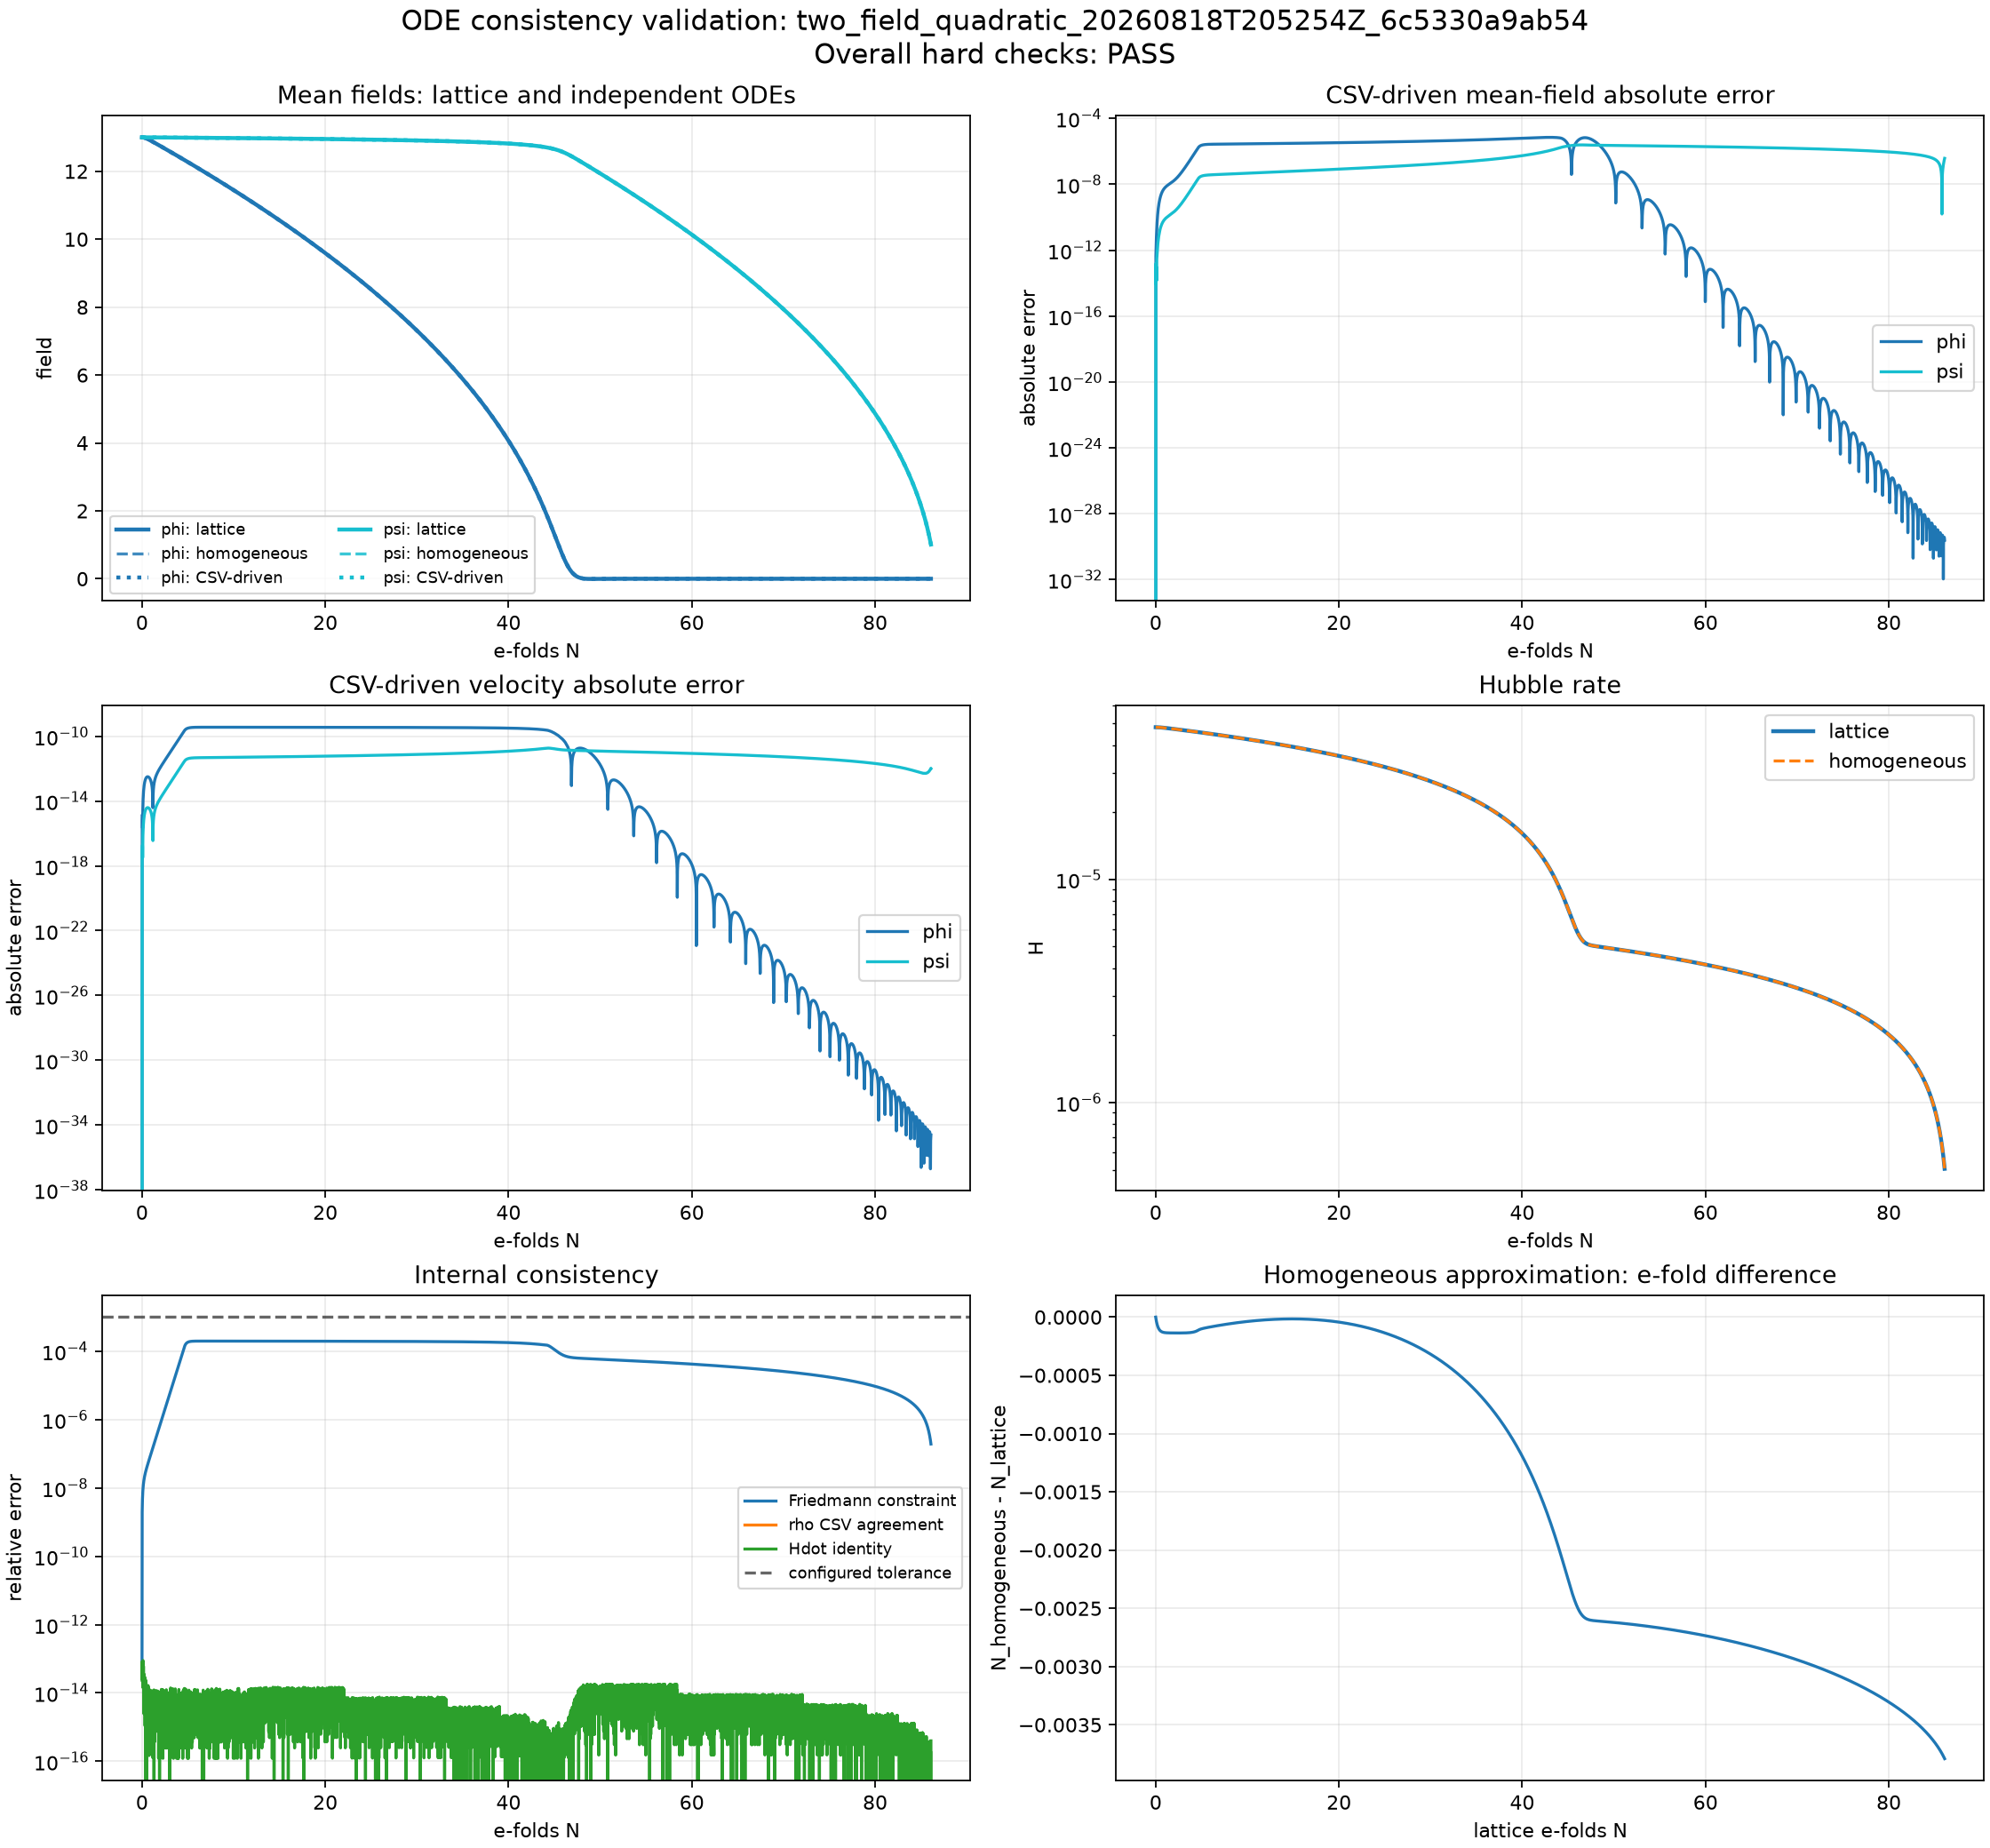
\includegraphics[height=0.88\textheight,keepaspectratio]{ode_consistency.png}
\caption{Pythonによる独立Dormand--Prince 5(4) ODEとの比較。CSV-driven解は平均場運動方程式を、一様場解はゆらぎエネルギーを除いた背景近似を検査する。}
\label{fig:ode}
\end{figure}

\begin{figure}[p]
\centering
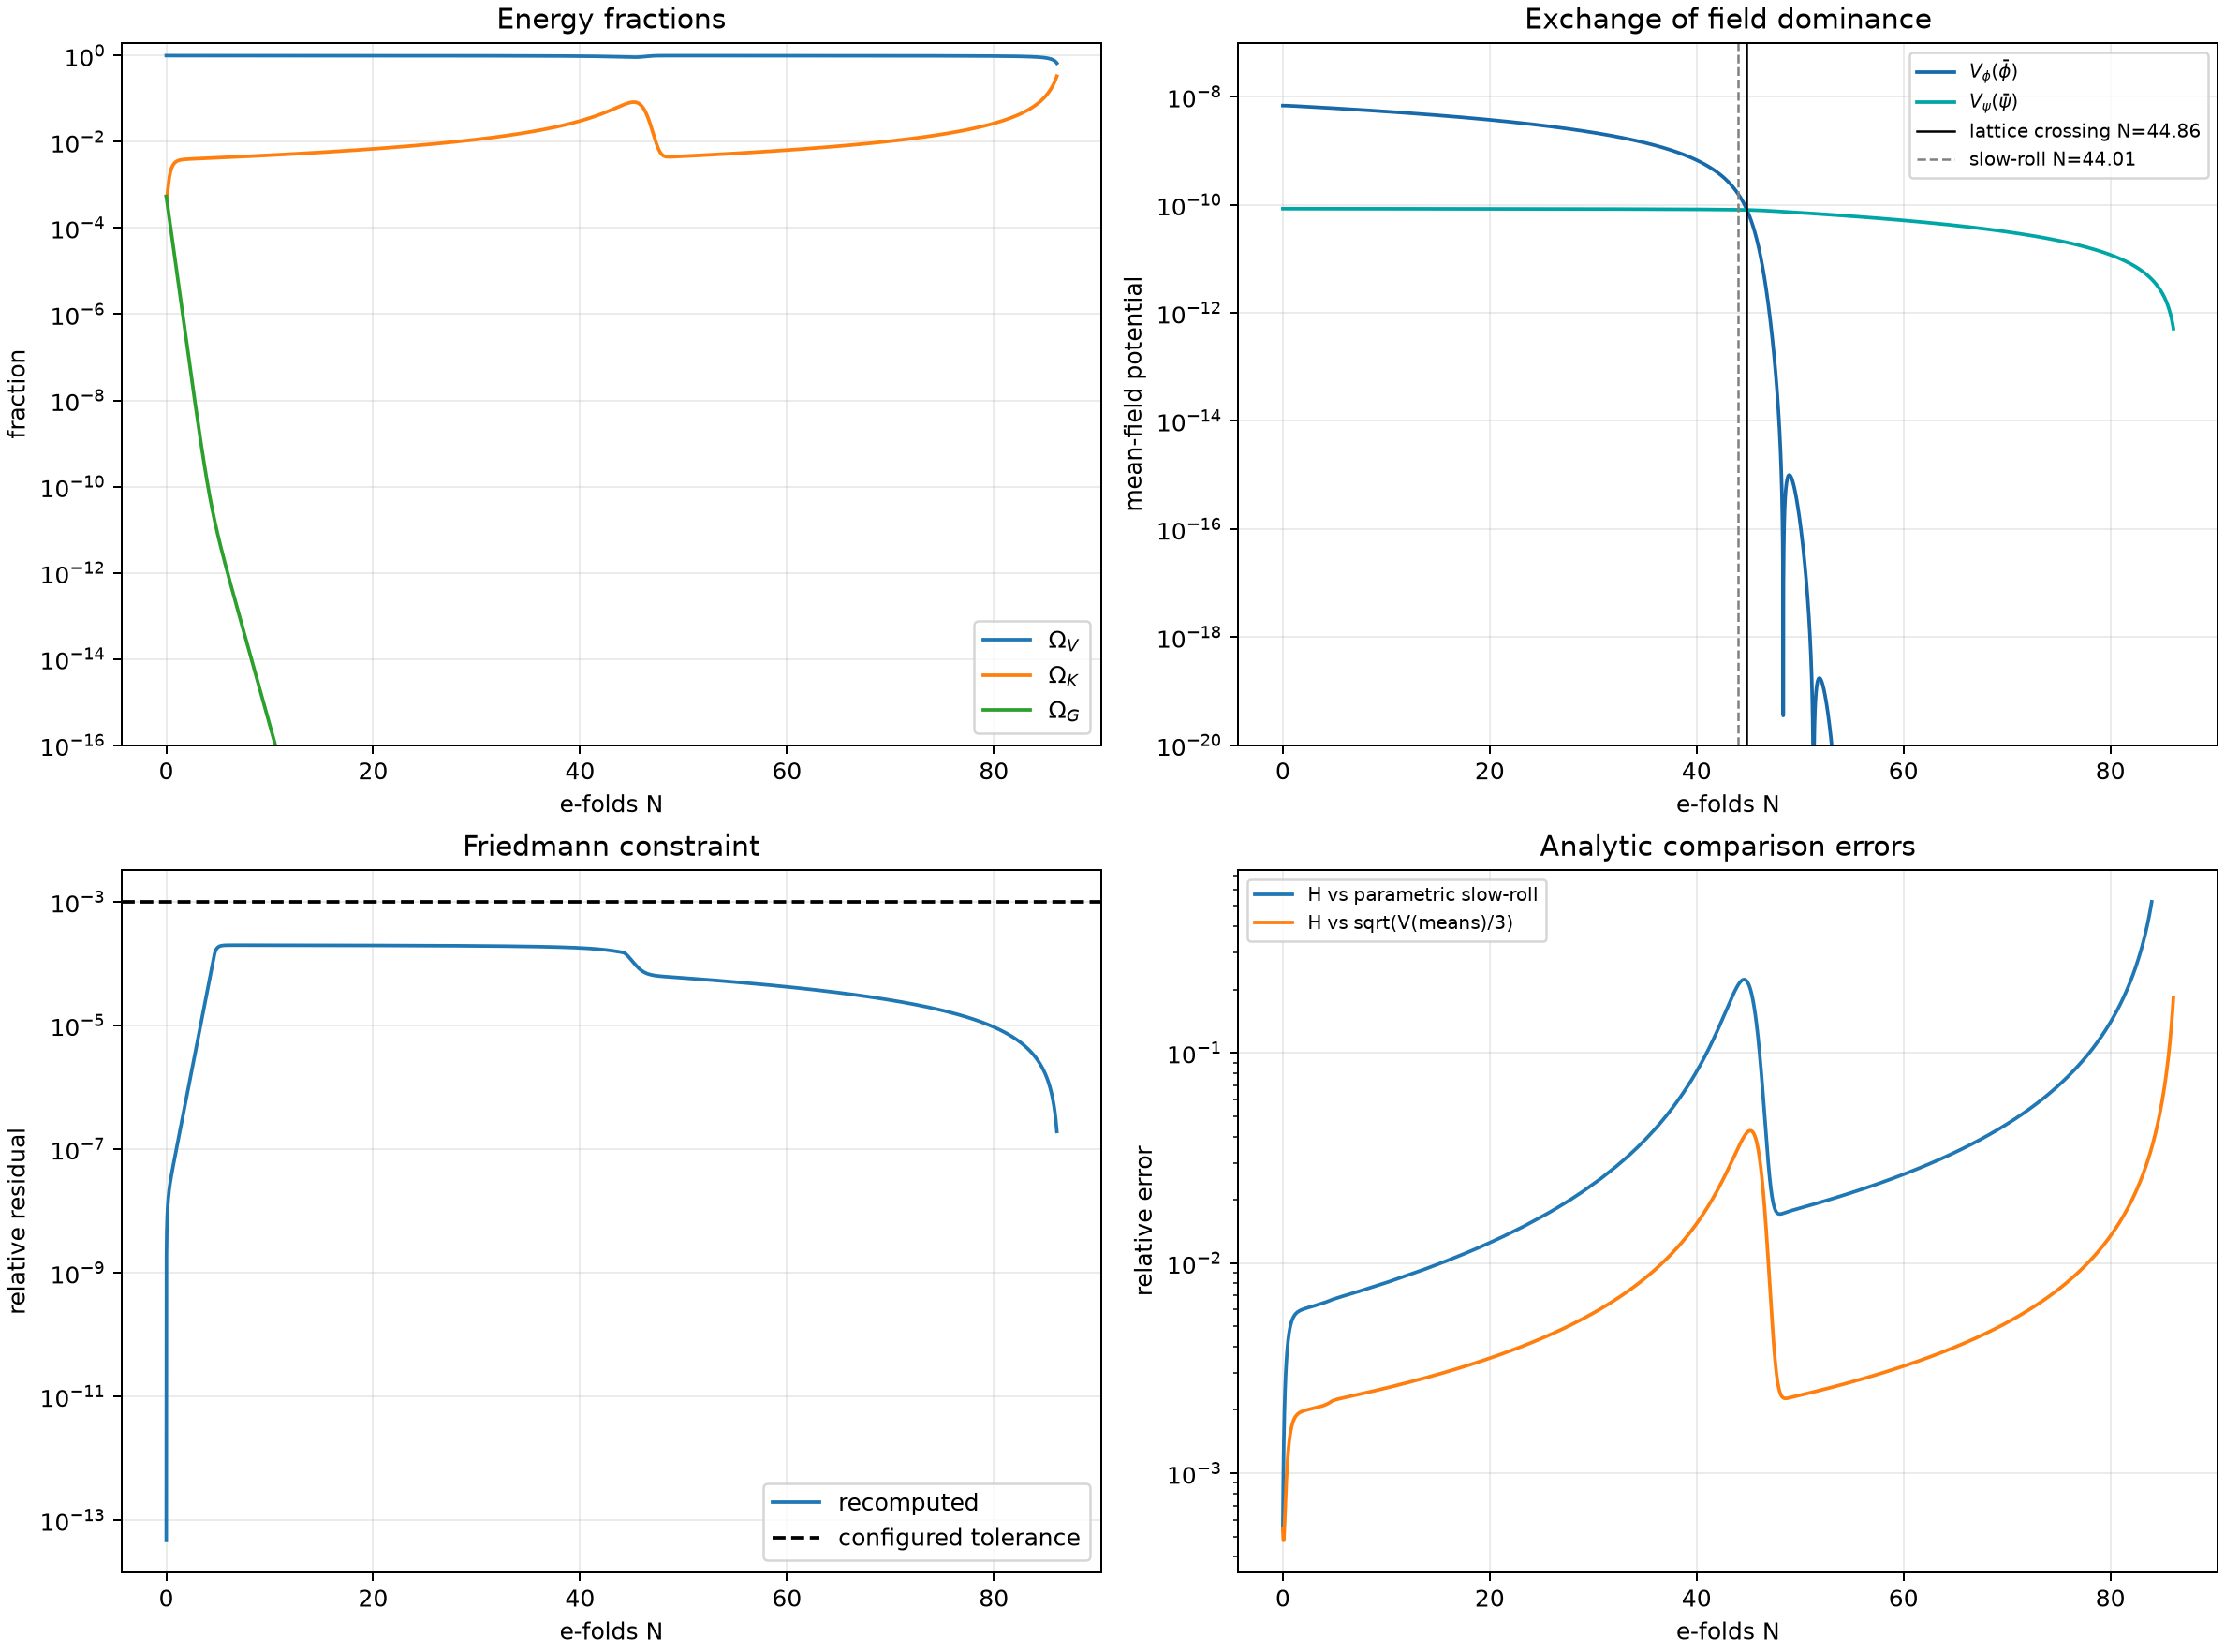
\includegraphics[width=0.98\textwidth]{energy_and_constraints.png}
\caption{エネルギー比、重い場から軽い場への支配交代、Friedmann拘束、および解析近似誤差。解析誤差の増加は主に場空間の曲がりと終了近傍に現れる。}
\label{fig:energy}
\end{figure}

\subsection{Bunch--Davies初期化とFFT規格化}

初期shell powerのBunch--Davies期待値に対するmode-weighted比は
$\phi$ で \num{\BDPhiWeightedRatio}、$\psi$ で
\num{\BDPsiWeightedRatio} である。軽い場の全sampled modeは
$N=\HorizonCrossingNMin$ から $\HorizonCrossingNMax$ の間に
Hubble crossingする。$N\simeq10$ で測定した十分なmode数
($n_{\mathrm{modes}}\geq50$)をもつ24 shellの
$\mathcal P_{\delta\psi}/(H_*/2\pi)^2$ は、平均
\num{\HorizonPsiMeanRatio}、中央値 \num{\HorizonPsiMedianRatio} であった。

スペクトル和と実空間分散の最大絶対差をpeak分散で規格化すると、
$\phi$ で \num{\ParsevalPhi}、$\psi$ で \num{\ParsevalPsi} である。
したがって真空振幅、Fourier規格化、shell集約と実空間分散は互いに整合する。
格子上のスカラー場計算とスペクトル規格化という検証観点は、既存の
expanding-universe lattice codeの方法論とも整合する\cite{FelderTkachev2008}。

\begin{figure}[p]
\centering
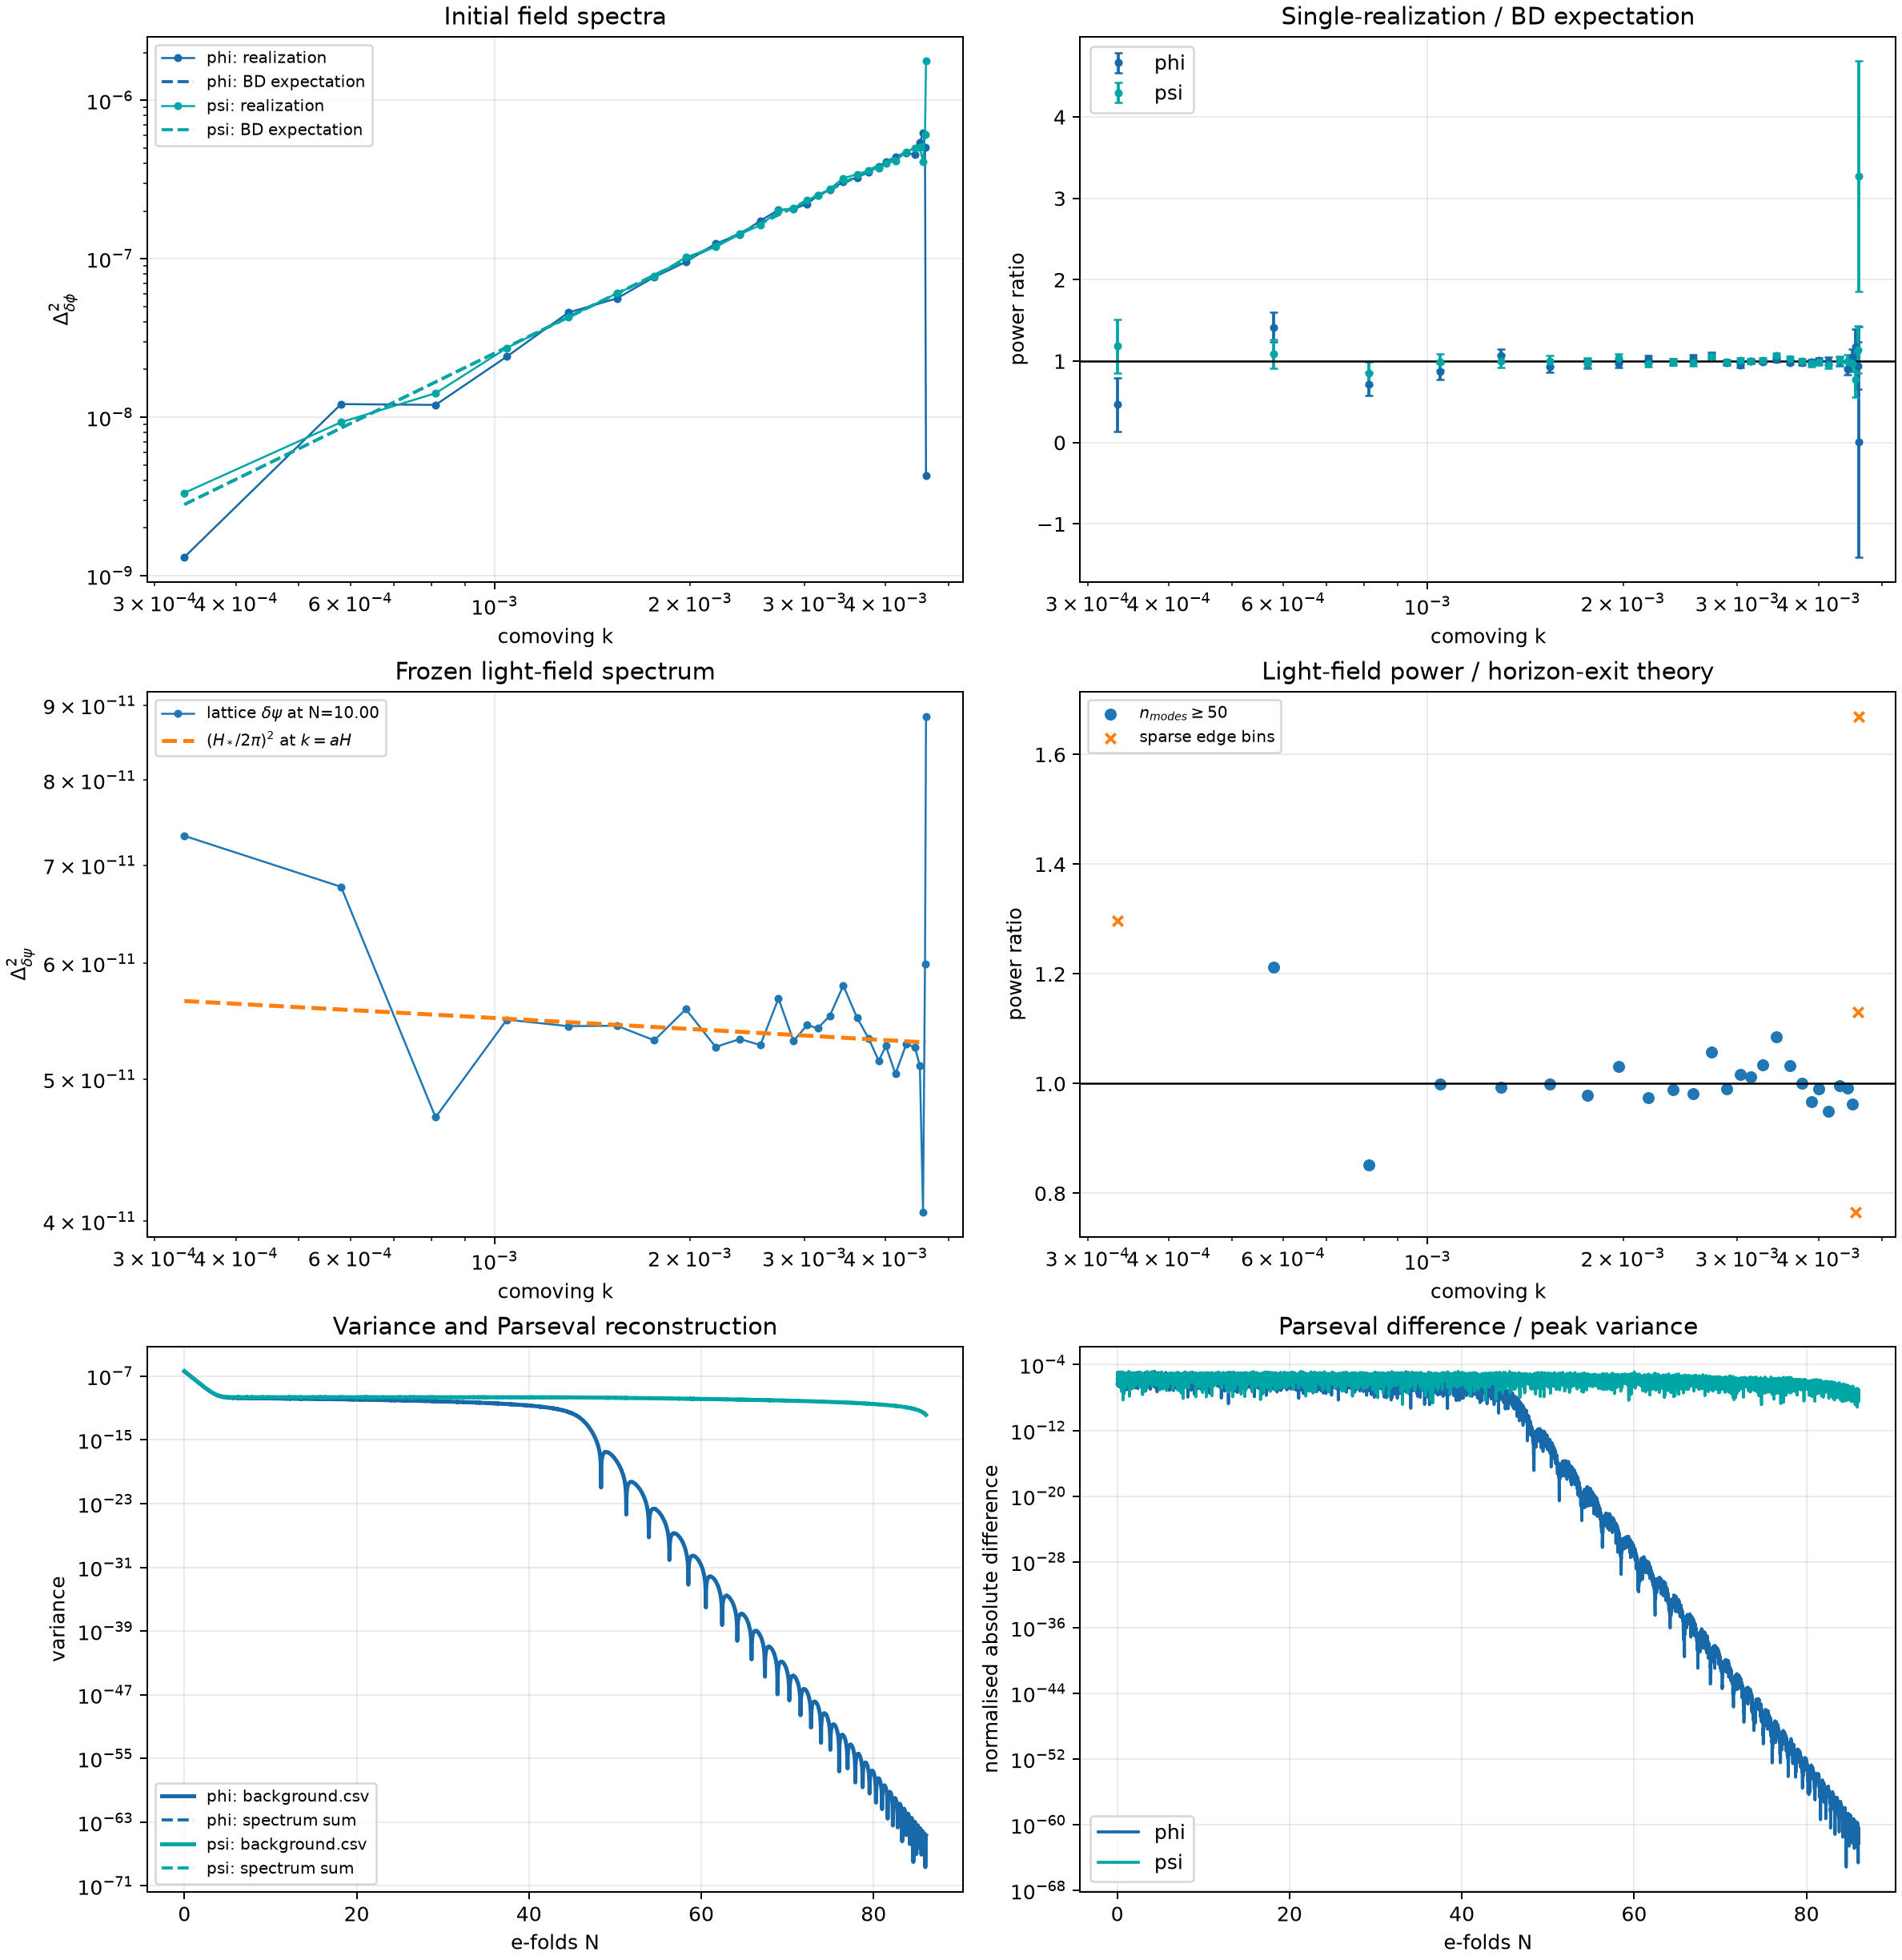
\includegraphics[height=0.90\textheight,keepaspectratio]{fluctuation_spectrum_checks.png}
\caption{上段: 初期Bunch--Daviesスペクトル。中段: 軽い場のfreeze-out振幅とHubble crossing時の解析予測。下段: Parseval再構成による分散とFFT規格化検査。edge shellはmode数が少ないため散乱が大きい。}
\label{fig:spectra}
\end{figure}

\section{判定表}

ここで使用した許容値は、本runの探索的妥当性確認のために事前に選んだ
実用的目安であり、普遍的な精度基準ではない。

\begin{table}[H]
\centering
\caption{主要検証項目。すべて選定許容値内である。}
\small
\begin{tabular}{p{0.39\textwidth}rrc}
\toprule
検証項目 & 測定値 & 許容値 & 判定 \\
\midrule
初期Hubble率の相対差 & \num{\InitialHRelativeDifference} & $10^{-2}$ & \pass \\
総e-fold数の相対差 & \num{\EfoldRelativeDifference} & $5\times10^{-2}$ & \pass \\
支配場交代時刻の相対差 & \num{0.0192277} & $10^{-1}$ & \pass \\
slow-roll $H$ 規格化RMS差 & \num{\HSRRms} & $5\times10^{-2}$ & \pass \\
slow-roll $\phi$ 規格化RMS差 & \num{\PhiSRRms} & $5\times10^{-2}$ & \pass \\
slow-roll $\psi$ 規格化RMS差 & \num{\PsiSRRms} & $5\times10^{-2}$ & \pass \\
最大Friedmann残差 & \num{\FriedmannMaximum} & $10^{-3}$ & \pass \\
slow-roll中の最大勾配比 & \num{\GradientFractionMaximum} & $10^{-2}$ & \pass \\
軽い場Hubble-exit power平均比の偏差 & \num{0.0041073} & $10^{-1}$ & \pass \\
Parseval差 ($\phi$, peak規格化) & \num{\ParsevalPhi} & $10^{-3}$ & \pass \\
独立ODE平均場RMS差 & \num{\ODEFieldRms} & $5\times10^{-4}$ & \pass \\
\bottomrule
\end{tabular}
\end{table}

\section{妥当性評価と限界}

本結果から、次の限定された結論は支持される。

\begin{quote}
単一格子・単一seedについて、格子平均された背景場、Hubble率、状態方程式、
総e-fold数および二場間の支配成分の交代は、二場二次ポテンシャルの
slow-roll予測と数percent以内で一致した。格子平均場は独立ODEと高精度で
一致し、Friedmann拘束とstress-energy分解は設定許容値内である。
さらに初期Bunch--Davies振幅、Hubble-exit後の軽い場スペクトル、および
Parseval再構成が解析予測と整合する。したがって本実装は、背景発展、
ゆらぎ初期化および場スペクトル規格化について、理論的に期待される
double-chaotic inflationの挙動を再現している。
\end{quote}

ただし、以下は本検証だけでは確立していない。

\begin{itemize}
  \item 時間刻み・空間解像度を変えた収束次数、連続極限、有限体積独立性。
  \item 複数seedによるensemble平均とスペクトルの統計誤差。
  \item metric perturbationを含む完全なMukhanov--Sasaki系との比較。
  \item \code{linear\_curvature\_spectra.csv} および
        \code{deltaN\_spectrum.csv} の独立な定量検証。
\end{itemize}

特にlinear curvature出力は、格子場と一様FLRW背景から後処理したproxyであり、
metric perturbationを動的に解いた結果ではない。またdelta-$N$ は終了時一様密度面と
最大1 e-foldのbackward範囲を使ったlate-time diagnosticである。これらをそのまま
保存されたprimordial curvature spectrumと同一視してはならない。さらに
メタデータには設定・manifest hashが保存されている一方、software commitは
\code{unknown} であり、厳密な版再現にはcommit記録を追加することが望ましい。

\section{再現方法}

解析コードはrun CSVを読み取り、図、比較時系列、判定CSV、JSON、TeX macroを
再生成する。プロジェクトの仮想環境で次を実行する。

\begin{verbatim}
.\.venv\Scripts\python.exe validation\20260818\compare_double_chaotic.py ^
  --project-root . ^
  --run runs\
two_field_quadratic_20260818T205254Z_6c5330a9ab54
\end{verbatim}

主な機械可読出力は
\code{data/validation\_metrics.csv},
\code{data/validation\_summary.json},
\code{data/analytic\_comparison\_timeseries.csv} である。
本TeXはLuaLaTeX環境で次のようにコンパイルできる。

\begin{verbatim}
cd report
lualatex double_chaotic_validation.tex
lualatex double_chaotic_validation.tex
\end{verbatim}

\section{結論}

解析的slow-roll軌道、初期Hubble率、二段階の支配交代、総e-fold数、
終了時の$\epsilon_H$と$w$、Friedmann拘束、独立ODE、Bunch--Davies振幅、
Hubble-exit後の軽い場power、およびParseval整合性は、互いに矛盾せず
選定許容値内で一致した。このため8月18日のrunは、背景および場ゆらぎ部門の
限定的な妥当性検証として説明可能である。次段階で必要なのは、より多くの
解析式を追加することより、格子解像度、時間刻み、box size、seedを変えた
収束・統計検証である。

\begin{thebibliography}{9}
\bibitem{Linde1983}
A. D. Linde,
``Chaotic Inflation,''
\textit{Physics Letters B} \textbf{129} (1983) 177--181,
\href{https://doi.org/10.1016/0370-2693(83)90837-7}{doi:10.1016/0370-2693(83)90837-7}.

\bibitem{Gordon2001}
C. Gordon, D. Wands, B. A. Bassett and R. Maartens,
``Adiabatic and entropy perturbations from inflation,''
\textit{Physical Review D} \textbf{63} (2001) 023506,
\href{https://arxiv.org/abs/astro-ph/0009131}{arXiv:astro-ph/0009131}.

\bibitem{FelderTkachev2008}
G. Felder and I. Tkachev,
``LATTICEEASY: A program for lattice simulations of scalar fields in an expanding universe,''
\textit{Computer Physics Communications} \textbf{178} (2008) 929--932,
\href{https://arxiv.org/abs/hep-ph/0011159}{arXiv:hep-ph/0011159}.
\end{thebibliography}

\end{document}
